\documentclass{article}

\usepackage{fullpage}
\usepackage{graphicx}
\usepackage{url}
\usepackage{amsmath}

\providecommand{\tightlist}{%
  \setlength{\itemsep}{0pt}\setlength{\parskip}{0pt}}

\author{Sergey Litvinov \and Lucas Amoudruz}
\title{Implementation of different DPD solvents in uDeviceX}
\date{}


\begin{document}
\maketitle

\section{Introduction}
We were working on \textit{uDeviceX}. We added restart option and
support of different ``colors'' of solvent particles.


\section{Restart}
The benefits of the restartable simulation are huge: computational
time is not wasted on transient part of the simulation, external and
not nececerly high performance tools can be used to
setup \texttt{uDeviceX} simulations, multi-stage simulations with very
different govering equations a every stage are possible, debuging and
testing is much simpler.

Restart is a dump of the state of \texttt{uDeviceX} simulation:
position of every solvent, wall, and RBC particles are dumped. State
of solid objects can be recovered from regular ``solid diag'' output.

See~\ref{a:restart} for the details of the restart file
organization. The format of the restart files is the same as for
output files and is described in~\ref{a:bop}. It does not use external
libraries and generation of such files is trivial in any programming
language.


\section{Colors}
Optional integer field ``color'' is attached to every solvent
particles. Force which acts between a pair of particles: ``A'' and
``B'' can be chosen based on the color of ``A'' and ``B''. For
example if conservative interaction is stronger in ``A'' - ``B'' pair
than in ``A'' - ``A'' and ``B'' - ``B'' pairs effective surface
tension force arises on the surface separation ``A'' and ``B''
region.

\texttt{uDeviceX} is also distinguishes between particles of different
kinds: ``wall'', ``RBC'', ``solvent'', ``solid''. The difference
between ``colors'' and ``kinds'' is that colors can be assigned
dynamically. Both ``kind'' and ``color'' can by used to choose between
different forces. For example, in pair ``solid'' - ``wall'' strong but
short range repulsive interaction is used.

See~\ref{a:color} for the details of how to use colors.


\section{Examples}
Examples of simulation using ``colors''.

\subsection{Double Poiseuille flow}
Domain is periodic and a hydrostatic force is acting in the direction of the arrows:
positive in one half of the domain and negative in the other half.  Red
particles are $100$ times for viscous. Particles are immiscible on the
right and fully miscible on the left. Arrows are velocity fields: red
particles have almost flat velocity profile.
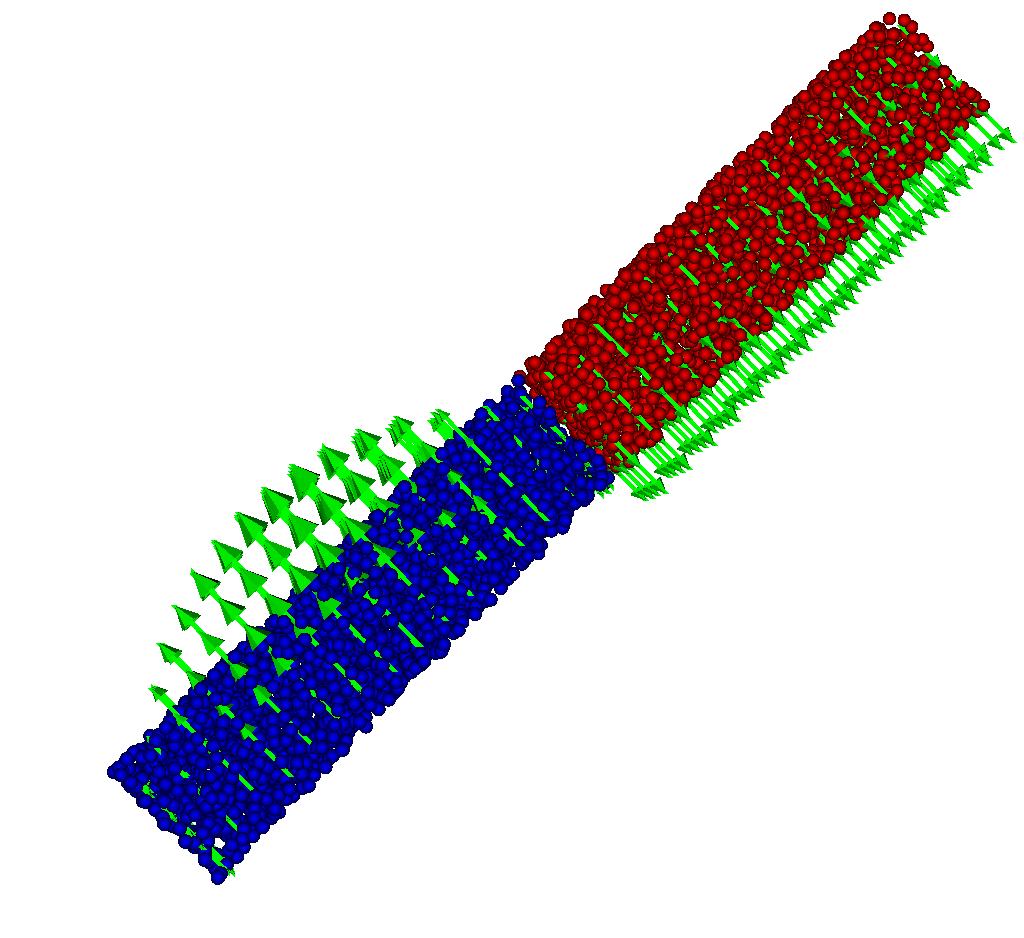
\includegraphics[width=0.5\textwidth]{i/flow/a/visit.png}
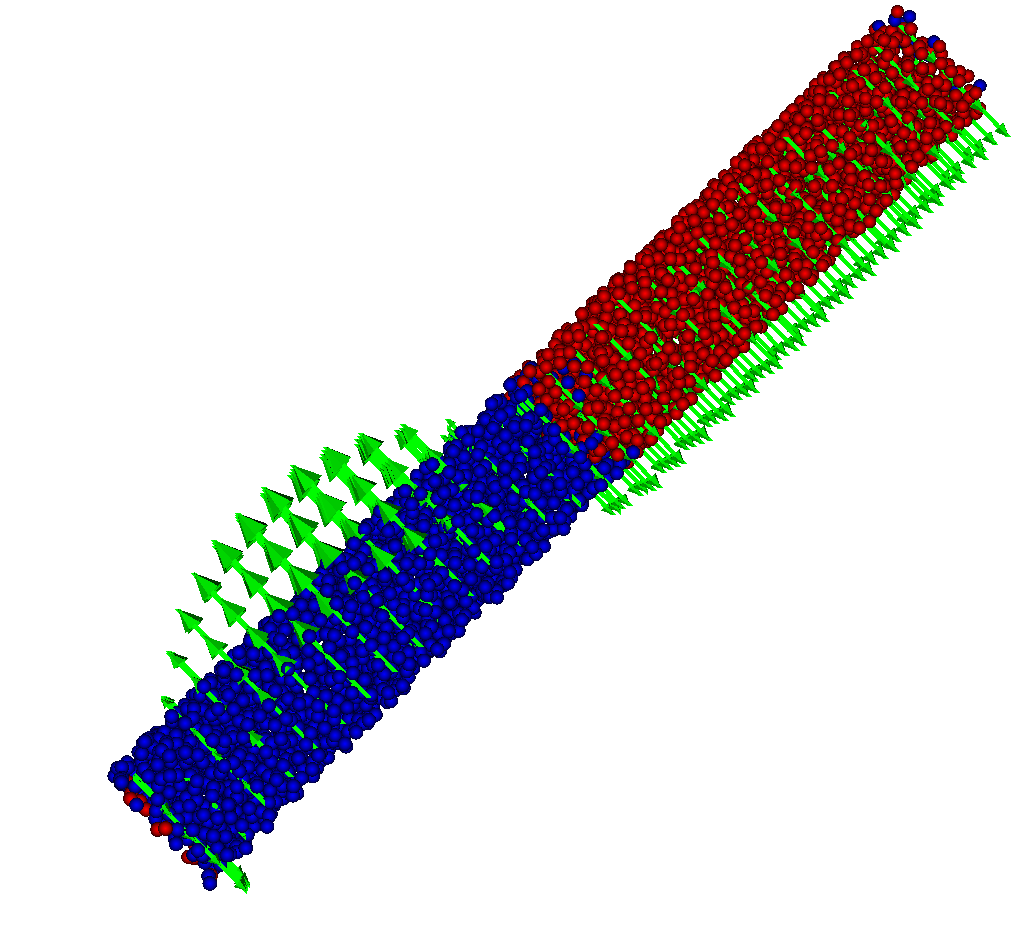
\includegraphics[width=0.5\textwidth]{i/flow/b/visit.png}


The average velocity fields are shown below. ``Immicible'' case is
more ``sharp''.

\begin{center}
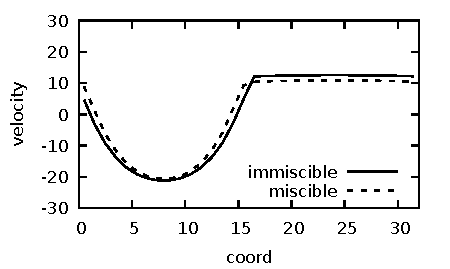
\includegraphics[width=0.6\textwidth]{i/flow/prof.pdf}
\end{center}


\subsection{Drops in double Poiseuille flow}
Viscous drop of immiscible liquid in double Poiseuille flow:
\begin{center}
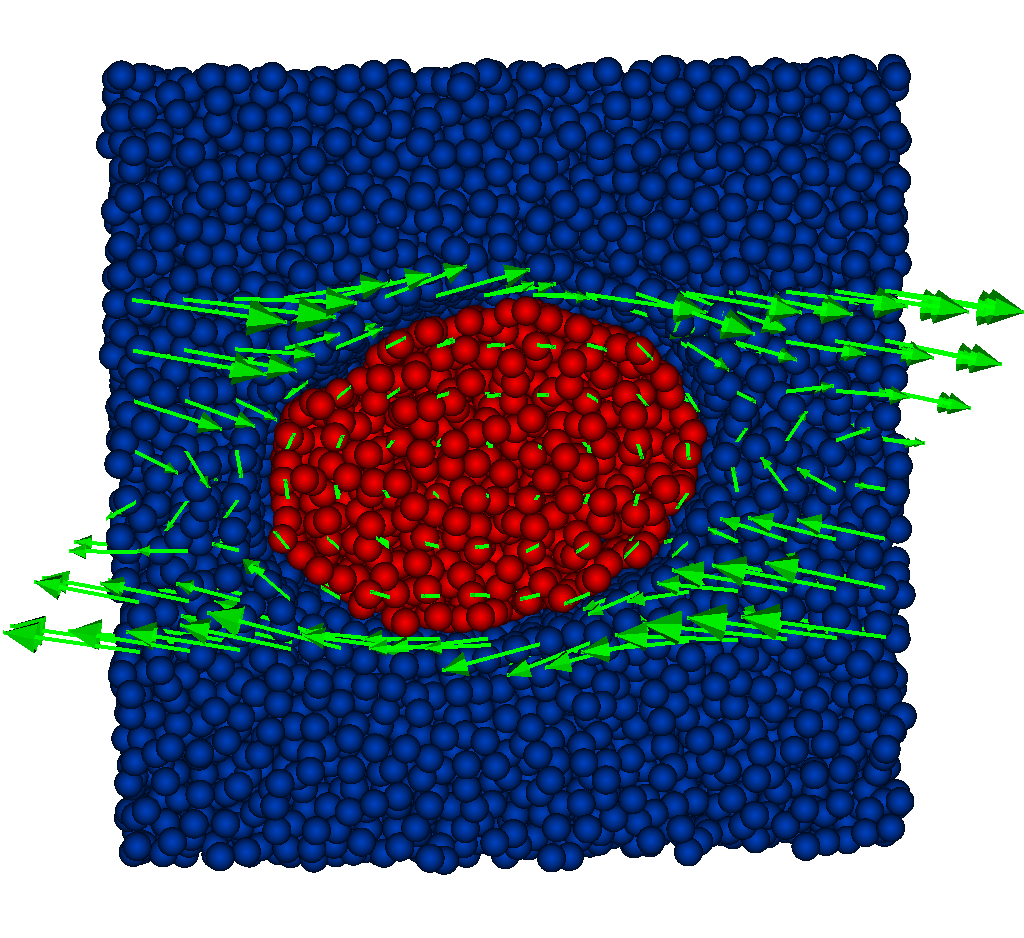
\includegraphics[width=0.6\textwidth]{i/drop/a/visit.png}
\end{center}

Viscous drop of miscible liquid in double Poiseuille flow.
\begin{center}
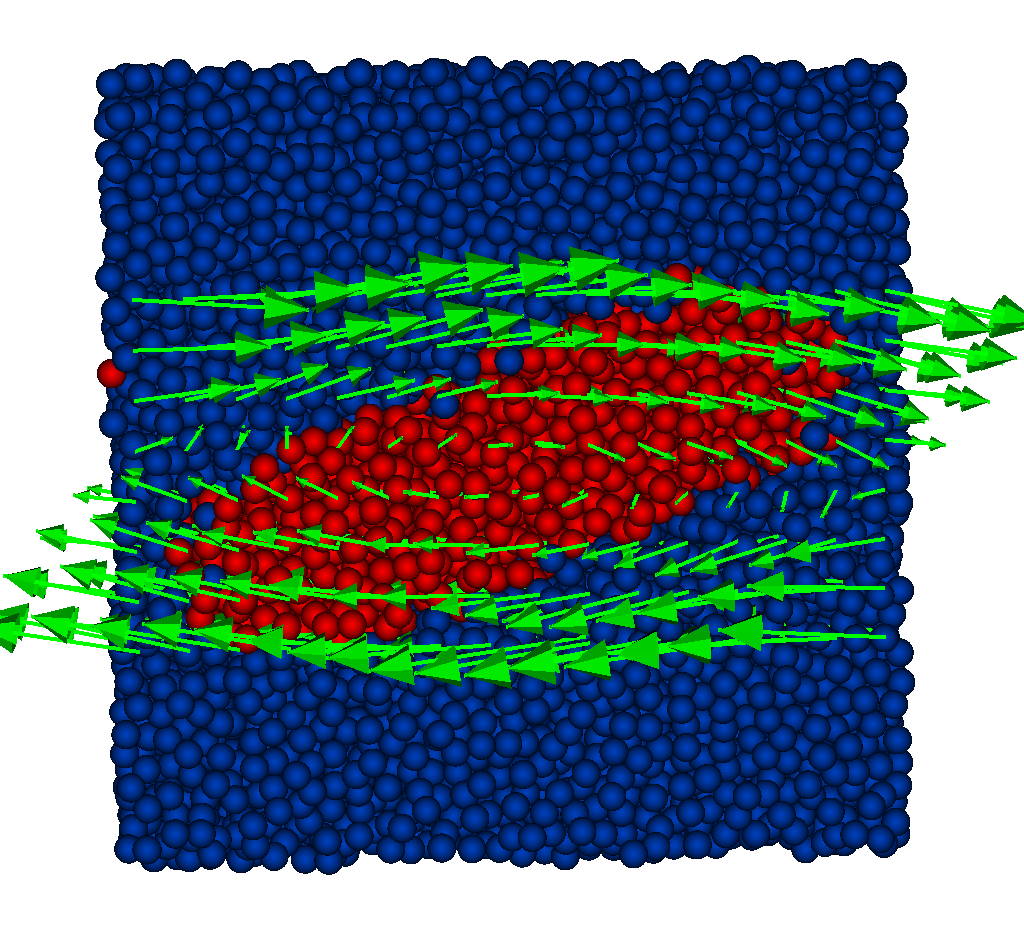
\includegraphics[width=0.6\textwidth]{i/drop/b/visit.png}
\end{center}


\subsection{Merging drops in double Poiseuille flow}
Two immiscible drops merging in double Poiseuille flow.
\begin{figure}
\begin{center}
\includegraphics[width=0.4\textwidth]{i/two/{visit.07}.png}
\includegraphics[width=0.4\textwidth]{i/two/{visit.10}.png}
\caption{Two drops in double Poiseuille flow. Left $t = 7$ DPD units, right $t = 10$ DPD units.}
\end{center}
\end{figure}


\appendix
\section{Restart}\label{a:restart}
Restart stores simulation variables of solvent, wall, rbcs and rigid
bodies under the following file naming:

\begin{verbatim}
strt/[code]/[XXX].[YYY].[ZZZ]/[ttt].[ext]
\end{verbatim}

where: * \texttt{{[}code{]}} is \texttt{flu} (solvent), \texttt{wall},
\texttt{rbc} or \texttt{rig} (rigid bodies) *
\texttt{{[}XXX{]}.{[}YYY{]}.{[}ZZZ{]}} are the coordinates of the
processor (no dir if single processor) * \texttt{{[}ttt{]}} is the id of
the restart; it has a magic value \texttt{final} for the last step of
simulation and is used to start from there. * \texttt{{[}ext{]}} is the
extension of the file: \texttt{bop} for particles, \texttt{ss} for
solids, \texttt{id.bop} for particle ids

Special case:

\begin{verbatim}
strt/[code]/[magic name].[ext]
\end{verbatim}

example: template frozen particles from rigid bodies or walls:
\texttt{templ}


\section{BOP (brick of particles)}\label{a:bop}
\subsection{Introduction}\label{introduction}

\texttt{file.bop} format (ascii, \texttt{\textless{}N\textgreater{}} is
the number of particles):

\begin{verbatim}
 <N>
 DATA_FILE: <file.values>
 DATA_FORMAT: <float|ascii|double|int|iascii>
 VARIABLES: <x> <y> <z> <vx> <vy> <vz> <id> ...
\end{verbatim}

\texttt{file.values} format:

\begin{verbatim}
x[0] y[0] z[0] vx[0] vy[0] vz[0] id[0]
...

x[N-1] y[N-1] ...
\end{verbatim}

The \texttt{ascii} format is assumed to be single precision floating
points data.\\
Th \texttt{iascii} format is the ascii version of integer data.

\subsection{Installation}\label{installation}

The following will install the binaries into \texttt{\$\{HOME\}/bin}.
This folder needs to be in the \texttt{PATH} variable. Furthermore, it
installs the headers and library into
\texttt{\$\{HOME\}/prefix/bop/include} and
\texttt{\$\{HOME\}/prefix/bop/lib}, respectively.

\begin{verbatim}
make && make install
\end{verbatim}

\subsection{Usage}\label{usage}

Convert bop files \texttt{in1.bop}, \texttt{in2.bop}, \ldots{},
\texttt{inN.bop} into a single vtk file \texttt{out.vtk}:

\begin{verbatim}
bop2vtk out.vtk in1.bop in2.bop ... inN.bop
\end{verbatim}

Dump ascii data from bop files \texttt{in1.bop}, \texttt{in2.bop},
\ldots{}, \texttt{inN.bop} into \texttt{out.txt}:

\begin{verbatim}
bop2txt in1.bop in2.bop ... inN.bop > out.txt
\end{verbatim}

\subsection{Testing}\label{testing}

Uses \texttt{atest} framework (https://gitlab.ethz.ch/mavt-cse/atest)

\begin{verbatim}
atest bop2txt.cpp
atest bop2vtk.cpp
\end{verbatim}


\section{Colors in \texttt{uDeviceX}}\label{a:color}
\subsection{colors}\label{colors}

Colors are activated by \texttt{\#define\ multi\_solvent\ true}.

Blue: represents outer solvent particles Red: represents inner solvent
particles

Color is an integer field. It is packed into \texttt{cloud.md} along
with \texttt{pp} arrays. Interactions (fsi, dpdl, dpdr, wall) get
\texttt{forces::Pa} from Clouds:

\begin{verbatim}
namespace forces {
struct Pa {
    float x, y, z, vx, vy, vz;
    int kind;
    int color;
};
\end{verbatim}

and passes it to \texttt{forces::gen}. See \texttt{src/forces/imp.h} which
decides which pair force to apply based on \texttt{int\ color}. It knows
about

\begin{verbatim}
enum {BLUE_COLOR, RED_COLOR};
\end{verbatim}

And miss-uses \texttt{gammadpd\_solv}, \texttt{gammadpd\_rbc} and
\texttt{gammadpd\_wall} to set DPD parameters for blue-blue, red-red,
and red-blue interactions.

In \texttt{sim::} colors are stored in

\begin{verbatim}
flu::QuantsI     qc;
\end{verbatim}

where

\begin{verbatim}
struct QuantsI {
    int *ii, *ii0;
    int *ii_hst;
 };
\end{verbatim}

in \texttt{sim::sim\_gen()} gets colors by calling

\begin{verbatim}
flu::gen_quants(&o::q, &o::qc);`
\end{verbatim}

which has a part different in different \texttt{u.md}. Hard-coded
color schemes are

\begin{itemize}
\tightlist
\item
  \texttt{flu/\_ussr} : all \texttt{BLUE\_COLOR} (default)
\item
  \texttt{flu/\_zurich} : flag of zurich in XY
\item
  \texttt{flu/\_bangladesh} : a sphere in the center
\item
  \texttt{flu/\_france} : flag of france in XY
\end{itemize}

Example \url{run/color/run}

\subsection{recolor}\label{recolor}

Re-coloring is done every \texttt{freq\_color} timesteps.
\texttt{freq\_color=0} means no re-coloring.


\end{document}
